% Options for packages loaded elsewhere
\PassOptionsToPackage{unicode}{hyperref}
\PassOptionsToPackage{hyphens}{url}
\PassOptionsToPackage{dvipsnames,svgnames,x11names}{xcolor}
%
\documentclass[
  letterpaper,
  DIV=11,
  numbers=noendperiod]{scrartcl}

\usepackage{amsmath,amssymb}
\usepackage{iftex}
\ifPDFTeX
  \usepackage[T1]{fontenc}
  \usepackage[utf8]{inputenc}
  \usepackage{textcomp} % provide euro and other symbols
\else % if luatex or xetex
  \usepackage{unicode-math}
  \defaultfontfeatures{Scale=MatchLowercase}
  \defaultfontfeatures[\rmfamily]{Ligatures=TeX,Scale=1}
\fi
\usepackage{lmodern}
\ifPDFTeX\else  
    % xetex/luatex font selection
  \setmainfont[]{Roboto-Regular.ttf}
\fi
% Use upquote if available, for straight quotes in verbatim environments
\IfFileExists{upquote.sty}{\usepackage{upquote}}{}
\IfFileExists{microtype.sty}{% use microtype if available
  \usepackage[]{microtype}
  \UseMicrotypeSet[protrusion]{basicmath} % disable protrusion for tt fonts
}{}
\makeatletter
\@ifundefined{KOMAClassName}{% if non-KOMA class
  \IfFileExists{parskip.sty}{%
    \usepackage{parskip}
  }{% else
    \setlength{\parindent}{0pt}
    \setlength{\parskip}{6pt plus 2pt minus 1pt}}
}{% if KOMA class
  \KOMAoptions{parskip=half}}
\makeatother
\usepackage{xcolor}
\setlength{\emergencystretch}{3em} % prevent overfull lines
\setcounter{secnumdepth}{-\maxdimen} % remove section numbering
% Make \paragraph and \subparagraph free-standing
\ifx\paragraph\undefined\else
  \let\oldparagraph\paragraph
  \renewcommand{\paragraph}[1]{\oldparagraph{#1}\mbox{}}
\fi
\ifx\subparagraph\undefined\else
  \let\oldsubparagraph\subparagraph
  \renewcommand{\subparagraph}[1]{\oldsubparagraph{#1}\mbox{}}
\fi


\providecommand{\tightlist}{%
  \setlength{\itemsep}{0pt}\setlength{\parskip}{0pt}}\usepackage{longtable,booktabs,array}
\usepackage{calc} % for calculating minipage widths
% Correct order of tables after \paragraph or \subparagraph
\usepackage{etoolbox}
\makeatletter
\patchcmd\longtable{\par}{\if@noskipsec\mbox{}\fi\par}{}{}
\makeatother
% Allow footnotes in longtable head/foot
\IfFileExists{footnotehyper.sty}{\usepackage{footnotehyper}}{\usepackage{footnote}}
\makesavenoteenv{longtable}
\usepackage{graphicx}
\makeatletter
\def\maxwidth{\ifdim\Gin@nat@width>\linewidth\linewidth\else\Gin@nat@width\fi}
\def\maxheight{\ifdim\Gin@nat@height>\textheight\textheight\else\Gin@nat@height\fi}
\makeatother
% Scale images if necessary, so that they will not overflow the page
% margins by default, and it is still possible to overwrite the defaults
% using explicit options in \includegraphics[width, height, ...]{}
\setkeys{Gin}{width=\maxwidth,height=\maxheight,keepaspectratio}
% Set default figure placement to htbp
\makeatletter
\def\fps@figure{htbp}
\makeatother

\newfontfamily\sectionfont{PixelOperatorSC.ttf}
\newfontfamily\subsectionfont{PixelOperatorSC.ttf}
\newfontfamily\subsubsectionfont{PixelOperatorSC.ttf}
\addtokomafont{section}{\sectionfont}
\addtokomafont{subsection}{\subsectionfont}
\addtokomafont{subsubsection}{\subsubsectionfont}
\usepackage{fontspec}
\usepackage{fancyhdr}
\usepackage{graphicx}
\usepackage{textpos}
\usepackage{background}
\usepackage[french]{babel}
\usepackage{datetime2}
\DTMsetdatestyle{french}
\pagestyle{fancy}
\usepackage[a4paper,margin=1.87cm,includefoot]{geometry}
\renewcommand{\headrulewidth}{0pt}
\newfontfamily\headerfont{PixelOperatorSC.ttf}
\fancyhead[L]{\headerfont CLESSN}
\fancyhead[C]{\headerfont Rapport présenté à Léger}
\fancyhead[R]{\headerfont Datagotchi Canada 2025}
\fancyfoot[C]{\vspace*{0.5cm}\thepage}
\KOMAoption{captions}{tableheading}
\makeatletter
\@ifpackageloaded{caption}{}{\usepackage{caption}}
\AtBeginDocument{%
\ifdefined\contentsname
  \renewcommand*\contentsname{Table of contents}
\else
  \newcommand\contentsname{Table of contents}
\fi
\ifdefined\listfigurename
  \renewcommand*\listfigurename{List of Figures}
\else
  \newcommand\listfigurename{List of Figures}
\fi
\ifdefined\listtablename
  \renewcommand*\listtablename{List of Tables}
\else
  \newcommand\listtablename{List of Tables}
\fi
\ifdefined\figurename
  \renewcommand*\figurename{Figure}
\else
  \newcommand\figurename{Figure}
\fi
\ifdefined\tablename
  \renewcommand*\tablename{Table}
\else
  \newcommand\tablename{Table}
\fi
}
\@ifpackageloaded{float}{}{\usepackage{float}}
\floatstyle{ruled}
\@ifundefined{c@chapter}{\newfloat{codelisting}{h}{lop}}{\newfloat{codelisting}{h}{lop}[chapter]}
\floatname{codelisting}{Listing}
\newcommand*\listoflistings{\listof{codelisting}{List of Listings}}
\makeatother
\makeatletter
\makeatother
\makeatletter
\@ifpackageloaded{caption}{}{\usepackage{caption}}
\@ifpackageloaded{subcaption}{}{\usepackage{subcaption}}
\makeatother
\ifLuaTeX
  \usepackage{selnolig}  % disable illegal ligatures
\fi
\usepackage{bookmark}

\IfFileExists{xurl.sty}{\usepackage{xurl}}{} % add URL line breaks if available
\urlstyle{same} % disable monospaced font for URLs
\hypersetup{
  colorlinks=true,
  linkcolor={blue},
  filecolor={Maroon},
  citecolor={Blue},
  urlcolor={Blue},
  pdfcreator={LaTeX via pandoc}}

\author{}
\date{}

\begin{document}

\begin{titlepage}
  \newfontfamily\titlepagefont{PixelOperatorSC.ttf}

  % Background image setup
  \backgroundsetup{
    scale=1.3,
    color=black,
    opacity=0.5,
    angle=0,
    position=current page.south,
    vshift=2.2cm,
    hshift=0cm,
    contents={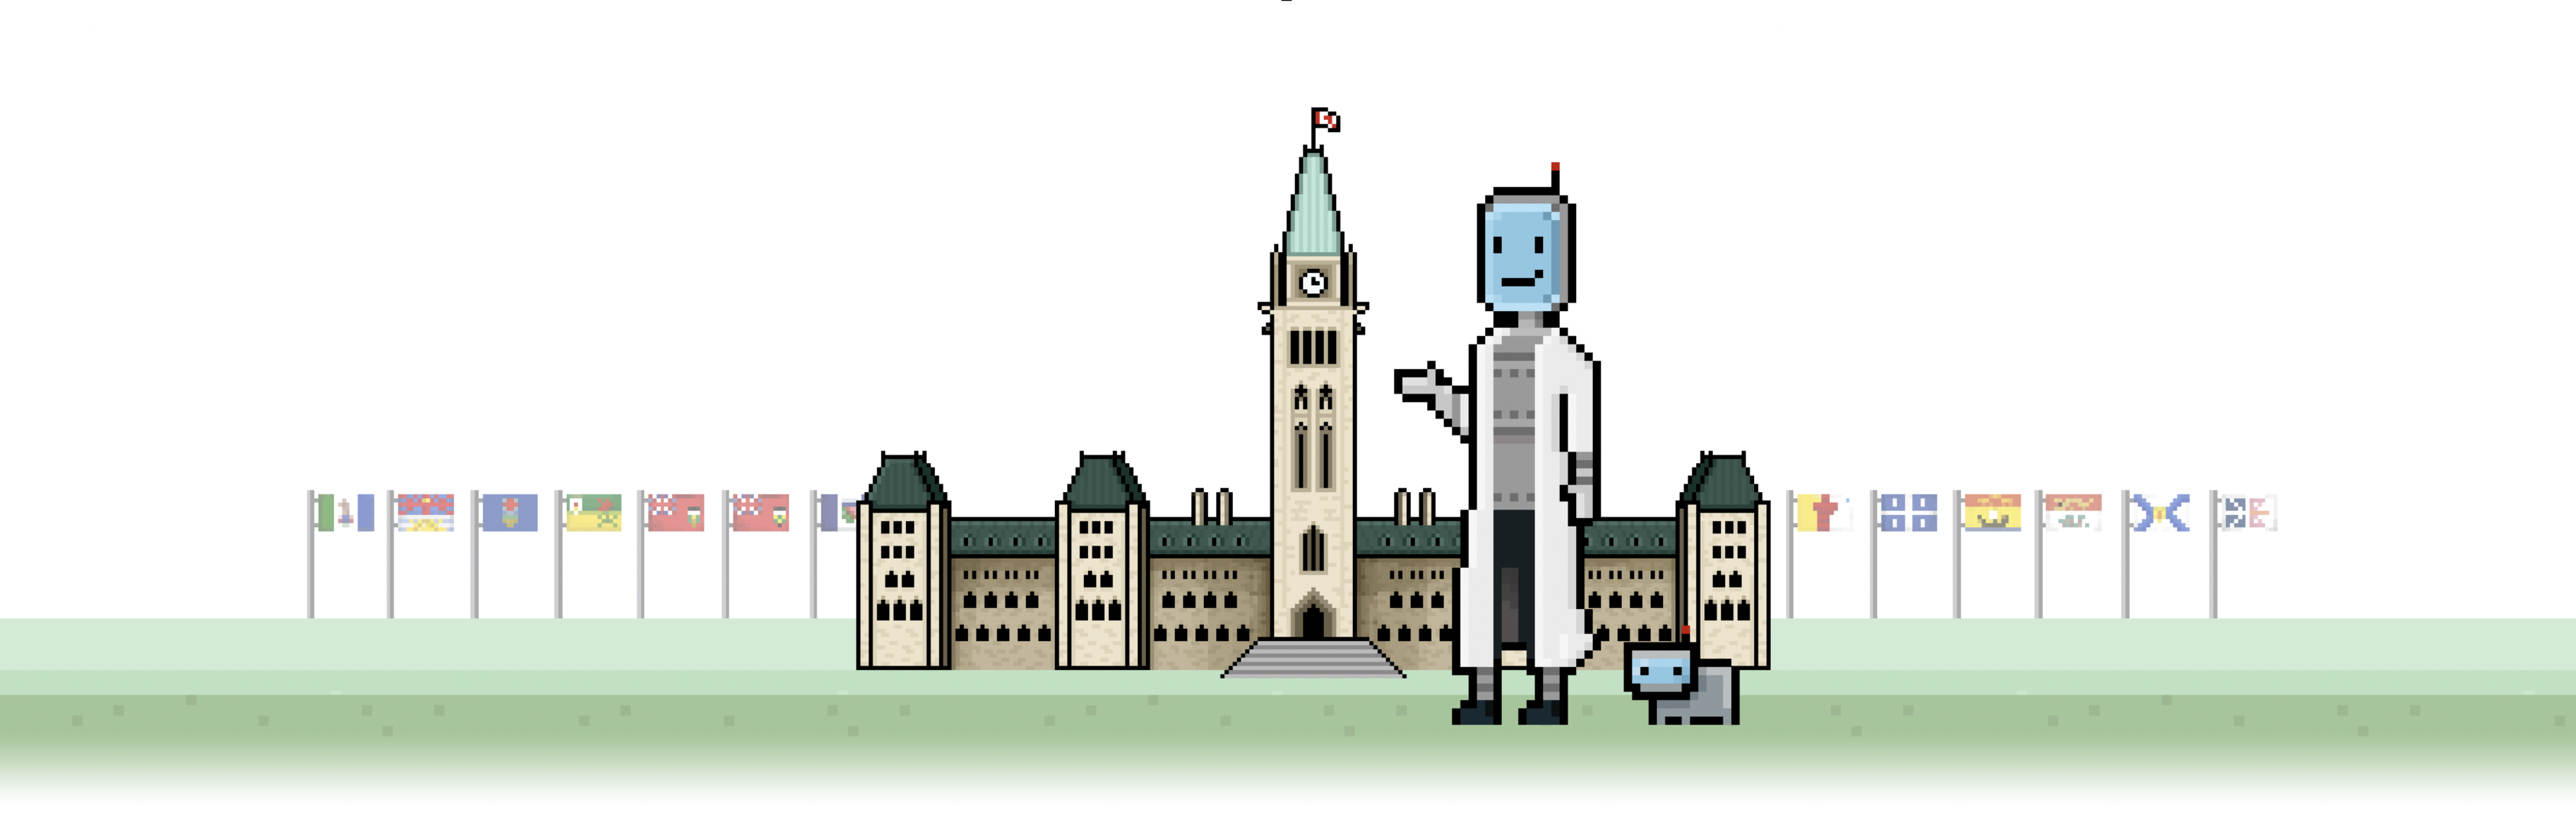
\includegraphics[width=1\textwidth]{img/datagotchi_canada.png}}
  }

  \begin{center}
    \null\vspace{\stretch{1}} % Ensures vertical centering
    {\titlepagefont\fontsize{48pt}{18pt}\selectfont \textbf{Léger-Datagotchi}}\\[1cm]
    {\titlepagefont\fontsize{32pt}{18pt}\selectfont \textbf{Rapport Canada 2025}}\\[1cm]
    
\includegraphics[width=0.2\textwidth]{img/leger_small.png}\\[1cm]
    {\titlepagefont\fontsize{32pt}{16pt}\selectfont \textbf{CLESSN}}\\[1cm]
    {\titlepagefont\fontsize{16pt}{14pt}\selectfont Rapport présenté à:}\\ % Smaller normal text size
    {\titlepagefont\fontsize{24pt}{16pt}\selectfont \textbf{Léger Marketing}}\\[1.5cm]
    {\titlepagefont\fontsize{16pt}{14pt}\selectfont Département de Science Politique\\Faculté des Sciences Sociales\\Université Laval}\\[2.5cm]
    {\titlepagefont\fontsize{16pt}{14pt}\selectfont Québec, Canada}\\[2cm]
    {\titlepagefont\fontsize{12pt}{12pt}\selectfont \copyright \thinspace CLESSN, \today}\\
    \null\vspace{\stretch{2}} % Ensures vertical centering
  \end{center}  \thispagestyle{empty} % Prevents headers and footers on the title page
  \clearpage % Ensures the next content starts on a clean page
\end{titlepage}
\backgroundsetup{contents={}}

\setcounter{page}{1}

\section{Description}\label{description}

Les ``Frat boys'' montrent une adhésion encore plus forte à l'idéologie
républicaine que les ``Rednecks'' eux-mêmes, avec une probabilité de 95
\% d'être totalement républicains, dépassant ainsi les 94 \% des
``Rednecks''. Ce paradoxe met en lumière une convergence inattendue
entre ces deux identités, où les stéréotypes sont inversés.

\begin{figure}[H]

{\centering 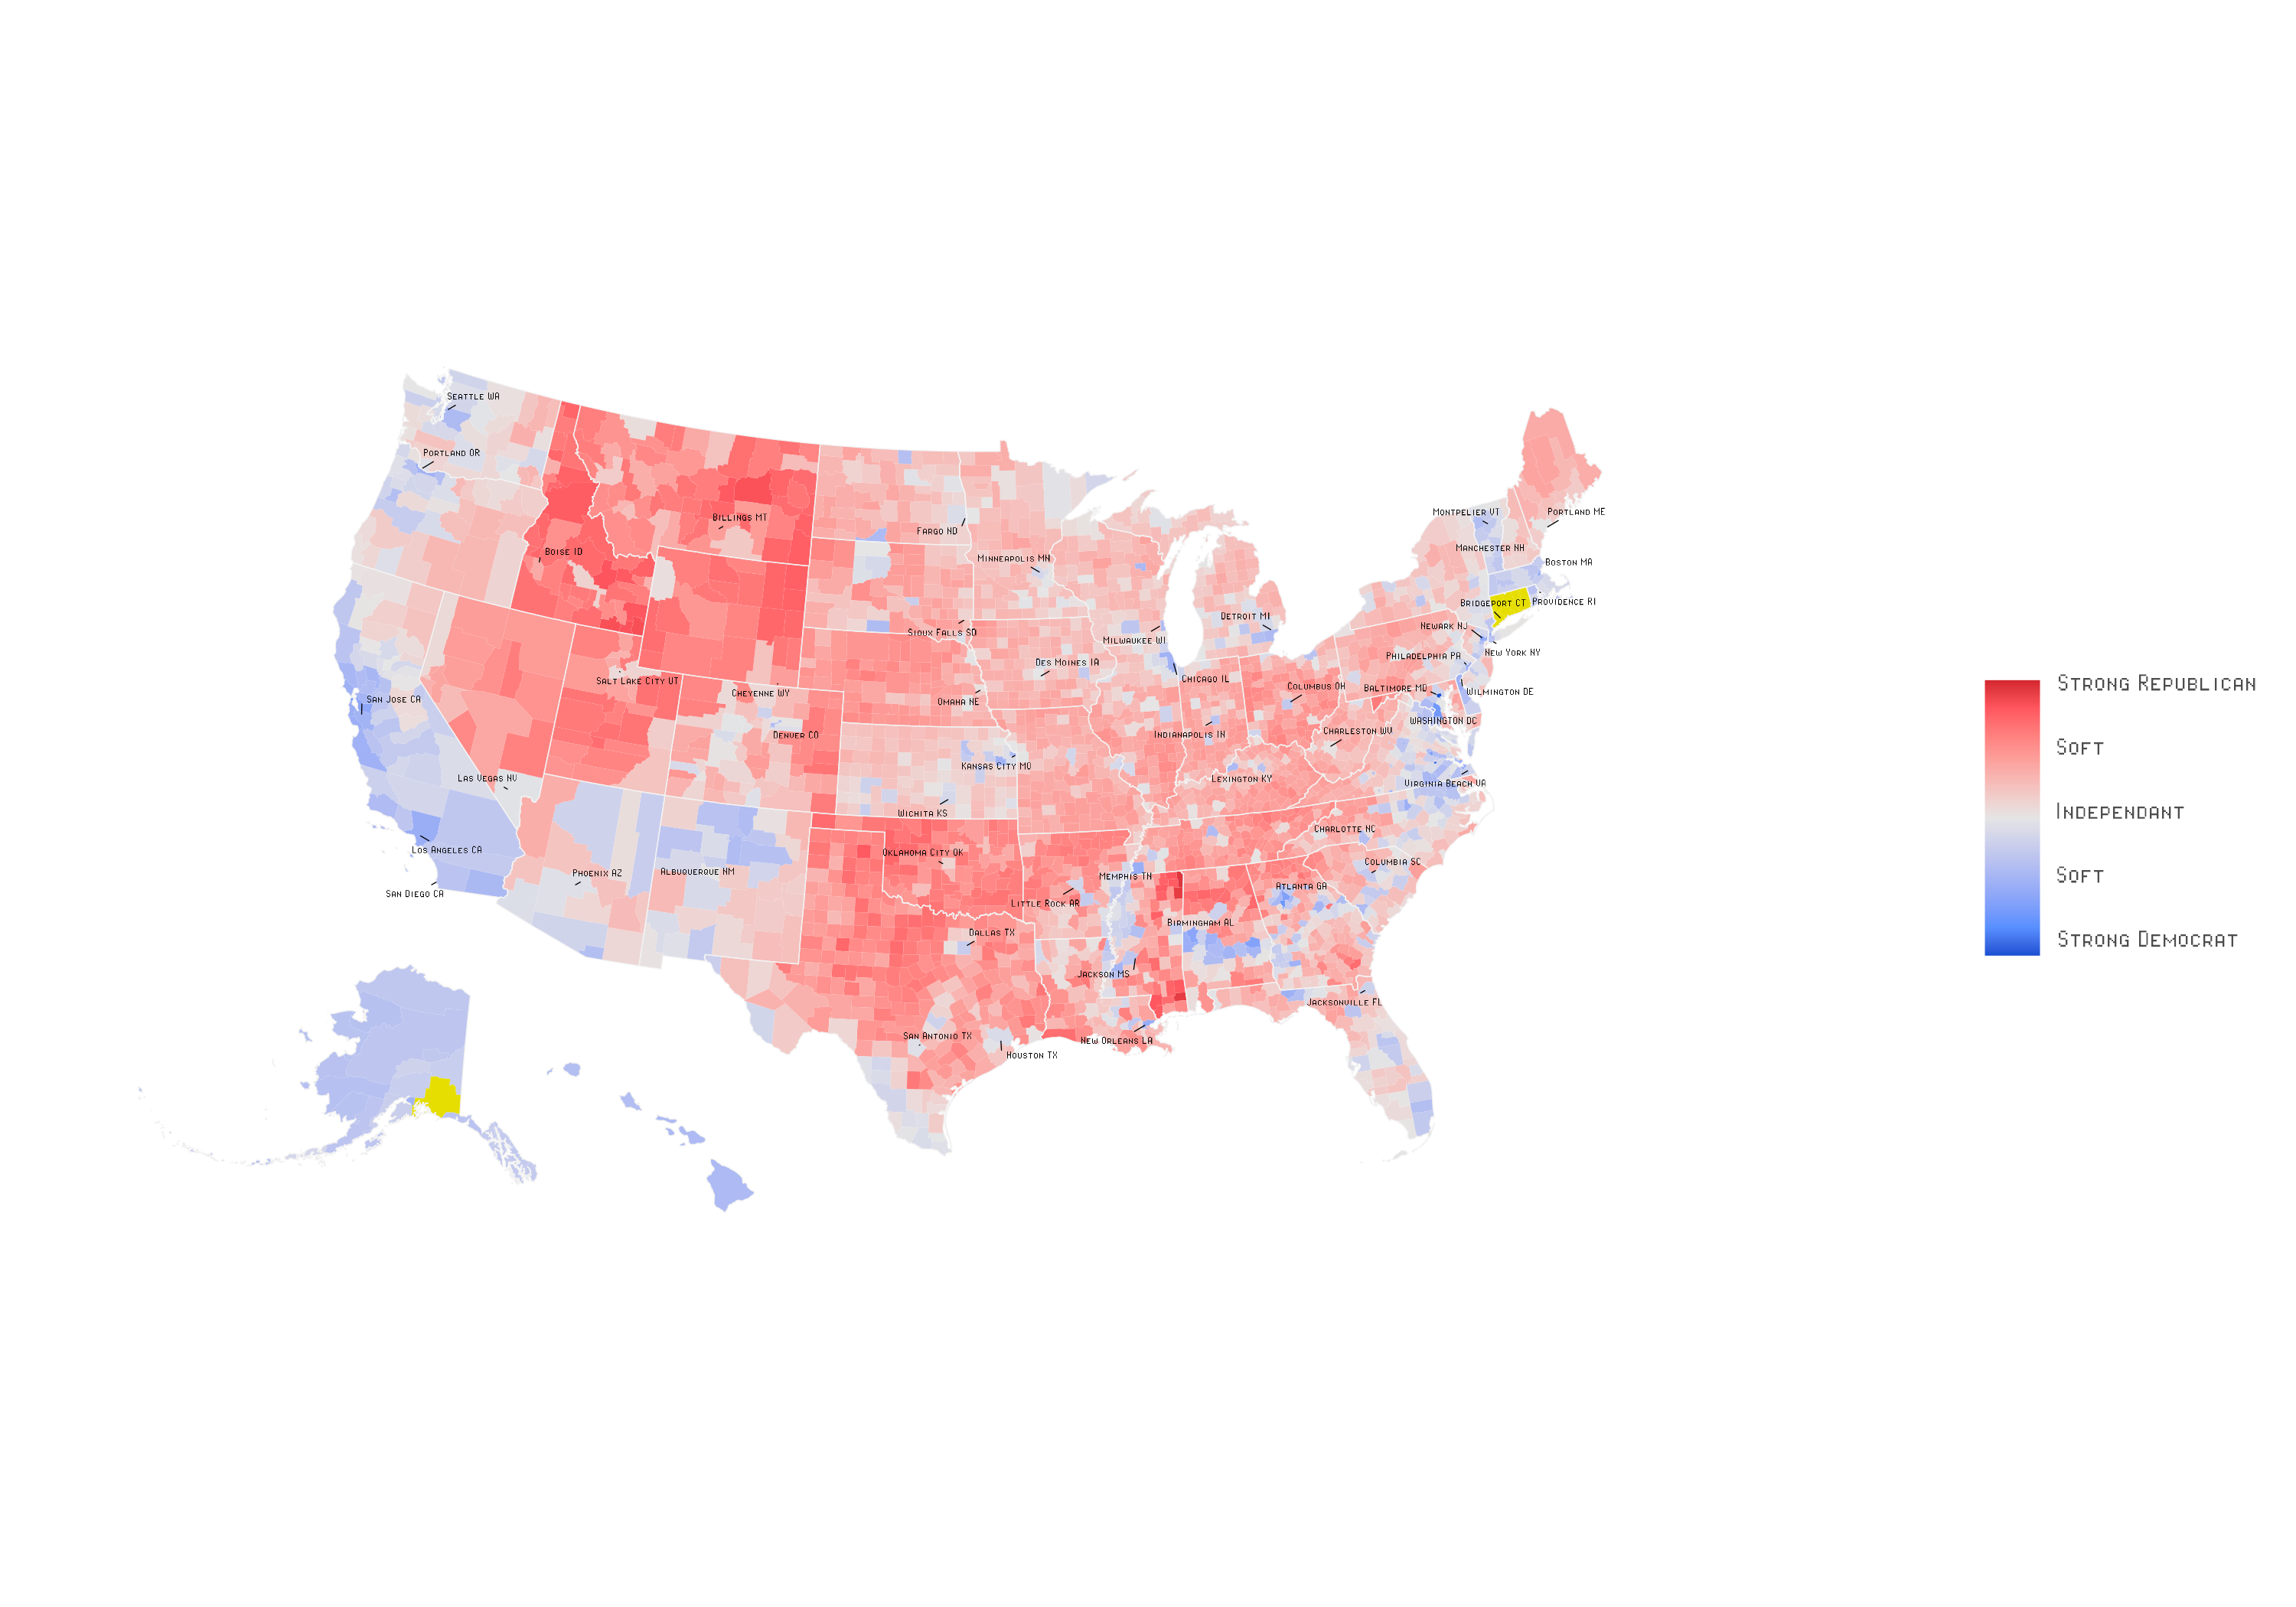
\includegraphics{img/graph_vote.png}

}

\caption{fratboys}

\end{figure}%



\end{document}
